\begin{enumerate}[label=\thesection.\arabic*.,ref=\thesection.\theenumi]
\numberwithin{equation}{enumi} 
\item The open loop transfer function of a feedback control system is  
\begin{align}
G(s) = \frac{1}{s(1+2s)(1+s)} 
\label{ee18btech11016_gs}
\end{align}
%
Find the magnitude and phase of $\abs{G\brak{\j\omega}}$.
\\
\solution
\begin{align}
G\brak{\j\omega} &= \frac{1}{\j\omega(1+2\j\omega)(1+\j\omega)} 
\\
 &= \frac{1}{\j\omega(1+3\j\omega-2\omega^2)}
\\
&=\frac{1}{\j\omega-3\omega^2-2\j\omega^3}
\\
 &= \frac{1}{-3\omega^2+\j\omega(1-2\omega^2)} 
\\
\implies \angle G\brak{\j\omega}&=- tan^{-1}\brak{\frac{\omega(1-2\omega^2)}{-3\omega^2}}
\label{ee18btech11016_gs_ang}
\end{align}
%
\item The frequency at which the phase of open-loop transfer function reaches -180$\degree$ or +180$\degree$ depending upon the range of tan inverse function) is defined to be the phase crossover frequency.  Find the phase crossover frequency for  \eqref{ee18btech11016_gs}.
\solution From \eqref{ee18btech11016_gs_ang}, at $\omega=\omega_{pc}$ 
\begin{align}
\omega(1-2\omega^2) = 0 
\\
\implies \omega_{pc} = \frac{1}{\sqrt{2}} 
\end{align}
\item The gain Margin is given by,
\begin{align}
GM = -20log_{10}\abs{G\brak{\j\omega_{pc}}} = 20log_{10}k_{g}
\end{align}
where 
\begin{align}
k_{g}=\frac{1}{\abs{G\brak{\j\omega_{pc}}}} 
\end{align}
%
Find the GM for \eqref{ee18btech11016_gs_ang}.
\\
\solution 
\begin{align}
\abs{G\brak{\j\omega_{pc}}} &= \frac{1}{\brak{\frac{3}{2}}}
\implies k_{g}&=\frac{1}{\abs{G\brak{\j\omega_{pc}}}} = \frac{3}{2}
3.5dB
\end{align}
The greater the Gain Margin (GM), the greater the stability of the system. The gain margin refers to the amount of gain, which can be increased or decreased without making the system unstable. It is usually expressed as a magnitude in dB.
\item Obtain the GM from the Bode plot.
\\
\solution The following code 
\begin{lstlisting}
codes/ee18btech11016.py
\end{lstlisting}
%
plots the amplitude and phase of \eqref{ee18btech11016_gs} in Fig. \ref{fig:ee18btech11016}.
%
\begin{figure}[htp]
	\centering
	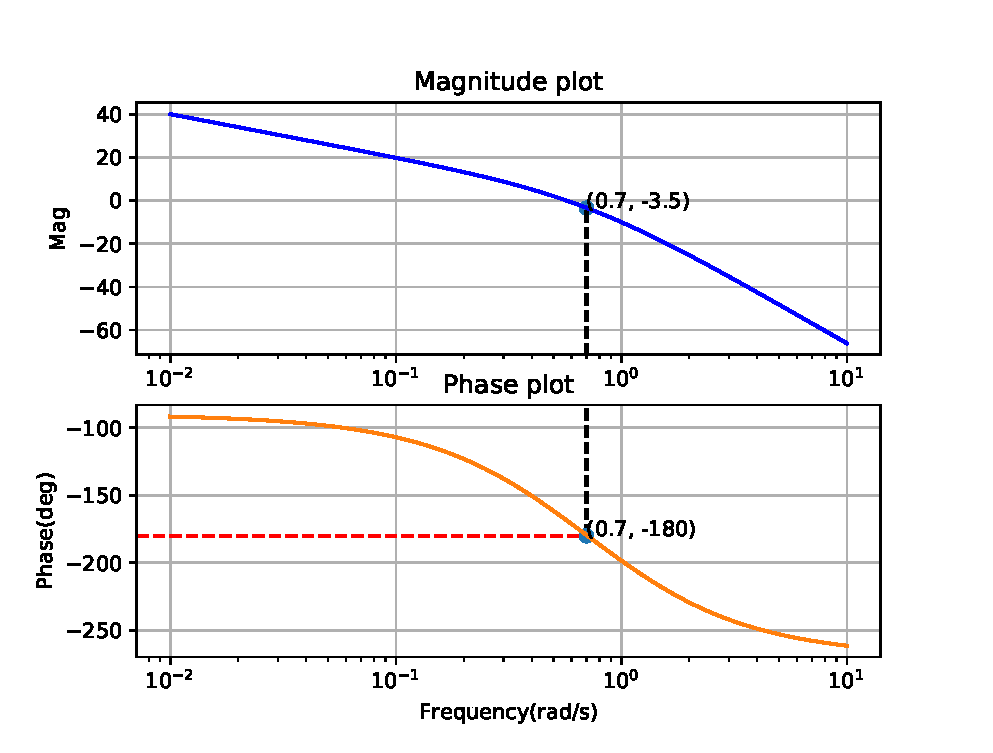
\includegraphics[width=\columnwidth]{./figs/ee18btech11016/ee18btech11016.eps}
	\caption{}
	\label{fig:ee18btech11016}
\end{figure}
From Fig. \ref{fig:ee18btech11016},
\begin{align}
20\log_{10}\abs{G\brak{\j\omega_{pc}}} &= -3.5dB,  \quad \omega_{pc} = -180\degree
\\
\implies  GM &= +3.5dB. 
\end{align}
\item A positive GM indicates closed loop stability with unity feedback.  Verify this for \eqref{ee18btech11016_gs}.
\\
\solution 
The characteristic equation is 
\begin{align}
1+G(s)=0 
\implies 2s^3 + 3s^2 + s + 1 = 0 
\end{align}
Constructing the routh array
\begin{align}
\mydet{s^3\\s^2\\s}
\mydet{2 & 1 & 0 \\ 3 & 1 & 0 \\ (1/3) & 0 & 0}
\\
\mydet{s^3\\s^2\\s\\s^0}
\mydet{2 & 1 & 0 \\ 3 & 1 & 0 \\ (1/3) & 0 & 0 \\ 1 & 0 & 0}
\end{align}\\
%
There are no sign changes in the first column of the routh array. 
$\therefore$ the system is stable.

\item Instead of unity feedback, consider a system with 
%
\begin{align}
H(s)=\frac{1}{s+1}
\end{align}
%
Find the magnitude and phase of $\abs{G\brak{\j\omega}H\brak{\j\omega}}$
\\
\solution 
%
\begin{align}
\because G(s)H(s) & =\frac{1}{s(1+2s)(s+1)^{2}},
\\
G\brak{\j\omega}H\brak{\j\omega} &= \frac{1}{(2\omega^4-4\omega^2) +j(\omega-5\omega^3)}
\\
\implies \angle G\brak{\j\omega}H\brak{\j\omega} &= -tan^{-1}(\frac{\omega-5\omega^3}{2\omega^4-4\omega^2})
\end{align}

\item Compute the open loop gain margin for this system.
\\
\solution 
For $\omega$=$\omega_{pc}$ 

\begin{align}
\text{Im}\cbrak{G\brak{\j\omega}H\brak{\j\omega}}&=0. 
\\
\implies\omega(1-5\omega^2)=0
\\
\implies\omega_{pc} = \frac{1}{\sqrt{5}}
\end{align}
Hence, 
\begin{align}
GM = -20log_{10}|G\brak{\j\omega_{pc}}H\brak{\j\omega_{pc}}| = 20log_{10}k_{g}
\end{align}
where 
\begin{align}
k_{g}&=\frac{1}{|G\brak{\j\omega_{pc}}H\brak{\j\omega_{pc}}|}
\\
&= \frac{ 18}{25} = 2.853dB.
\end{align}
%
Hence $GM < 0$ and the system is unstable.
%
\item Obtain the GM from the Bode plot.
\\
\solution The following code 
\begin{lstlisting}
codes/ee18btech11016_2.py
\end{lstlisting}
%
plots the amplitude and phase of \eqref{ee18btech11016_gs} in Fig. \ref{fig:ee18btech11016_2}.
%
\begin{figure}[htp]
	\centering
	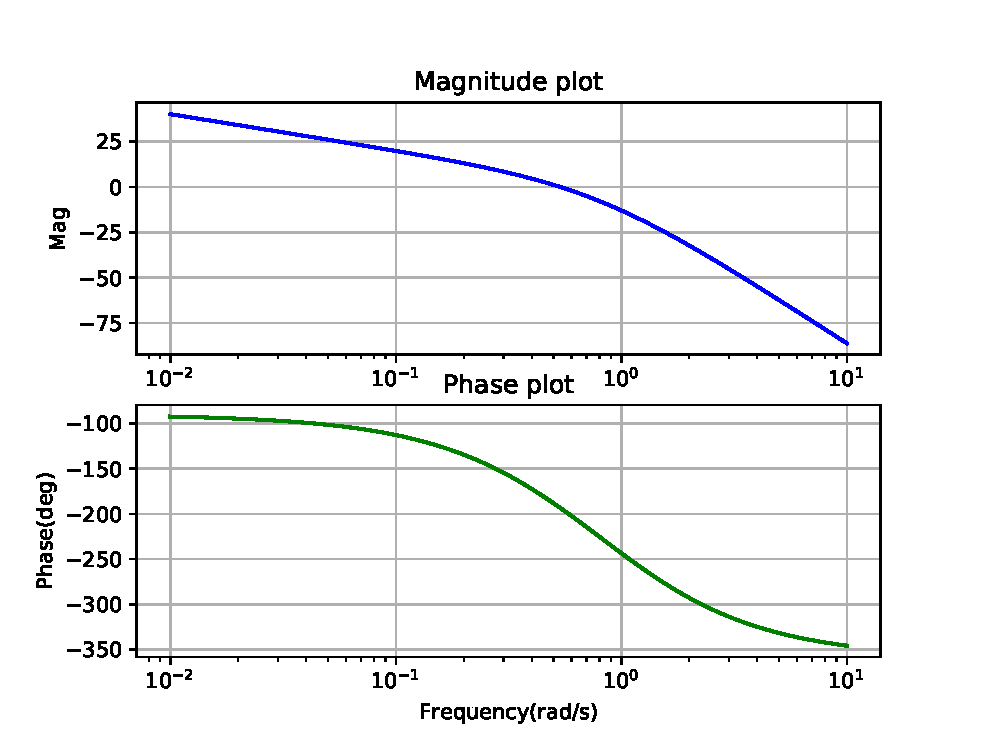
\includegraphics[width=\columnwidth]{./figs/ee18btech11016/ee18btech11016_2.eps}
	\caption{}
	\label{fig:ee18btech11016_2}
\end{figure}
\item Show that the closed loop transfer function 
\begin{align}
T(s) = \frac{1}{1 + (s(1+2s)(1+s)^2)}
\end{align}
%
is unstable using the Routh Hurwitz criterion.
\\
\solution 
The characteristics equation is 
\begin{align}
2s^4 + 5s^3 + 4s^3 + s + 1 = 0 
\end{align}
Constructing routh array for the above,
\begin{align}
\mydet{s^4\\s^3\\s^2}
\mydet{2 & 4 & 1 \\ 5 & 1 & 0 \\ (18/5) & 1 & 0}
\\
\mydet{s^4\\s^3\\s^2\\s}
\mydet{2 & 1 & 0 \\ 3 & 1 & 0 \\ (18/5) & 1 & 0 \\ (-7/18) & 0 & 0}
\\
\mydet{s^4\\s^3\\s^2\\s\\s^0}
\mydet{2 & 1 & 0 \\ 3 & 1 & 0 \\ (18/5) & 1 & 0 \\ (-7/18) & 0 & 0 \\ 1 & 0 & 0}
\end{align}
%
There are 2 sign changes in the first column of the routh array. So, 2 poles lie on right half of s-plane.
Therefore,the system is unstable.
%
\end{enumerate}


